% Appendix Template

\chapter{CFD validation} % Main appendix title

\label{cfd_results} % Change X to a consecutive letter; for referencing this appendix elsewhere, use \ref{AppendixX}
\fancyhead[RE, LO]{\emph{CFD validation}} % Change X to a consecutive letter; this is for the header on each page - perhaps a shortened title

%S10P20
\begin{figure}[ht]
  \centering
  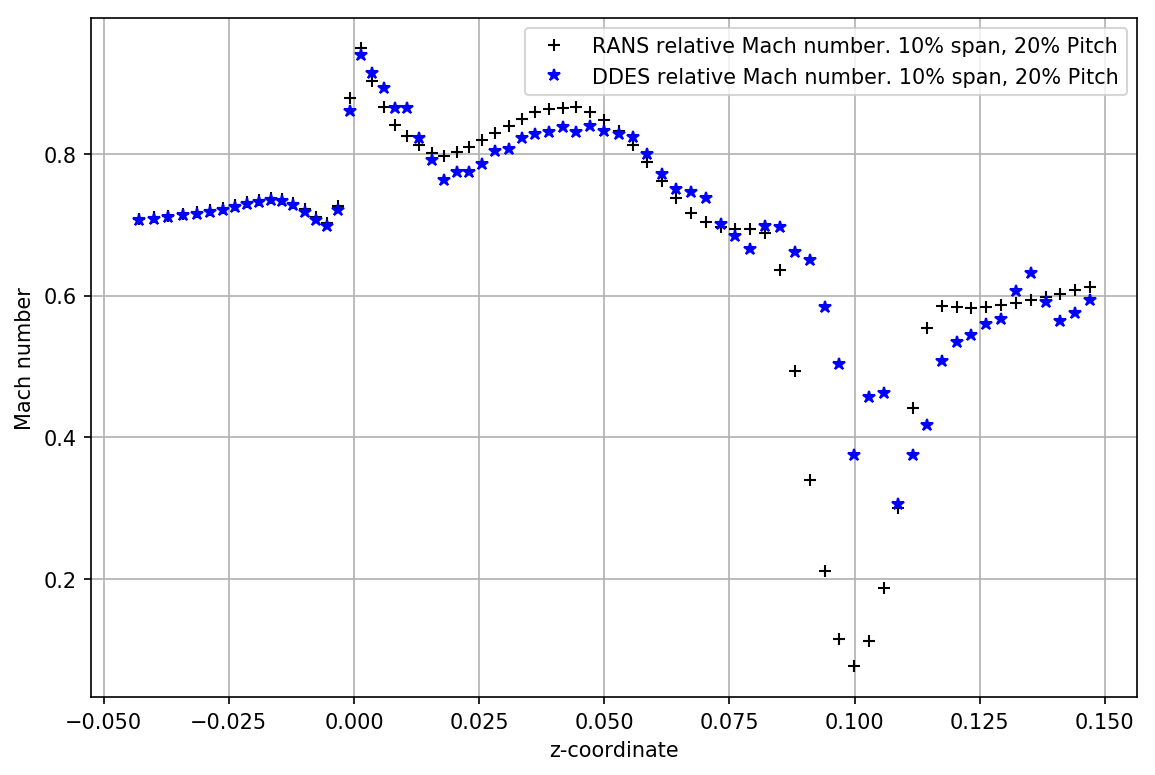
\includegraphics[width=0.7\textwidth]{Pictures/mach-rel-S10-P20.png}
  \caption{Relative Mach number at S10P20 streamline} \label{mach-rel-S10-P20}  
  \vspace*{\floatsep}% https://tex.stackexchange.com/q/26521/5764
  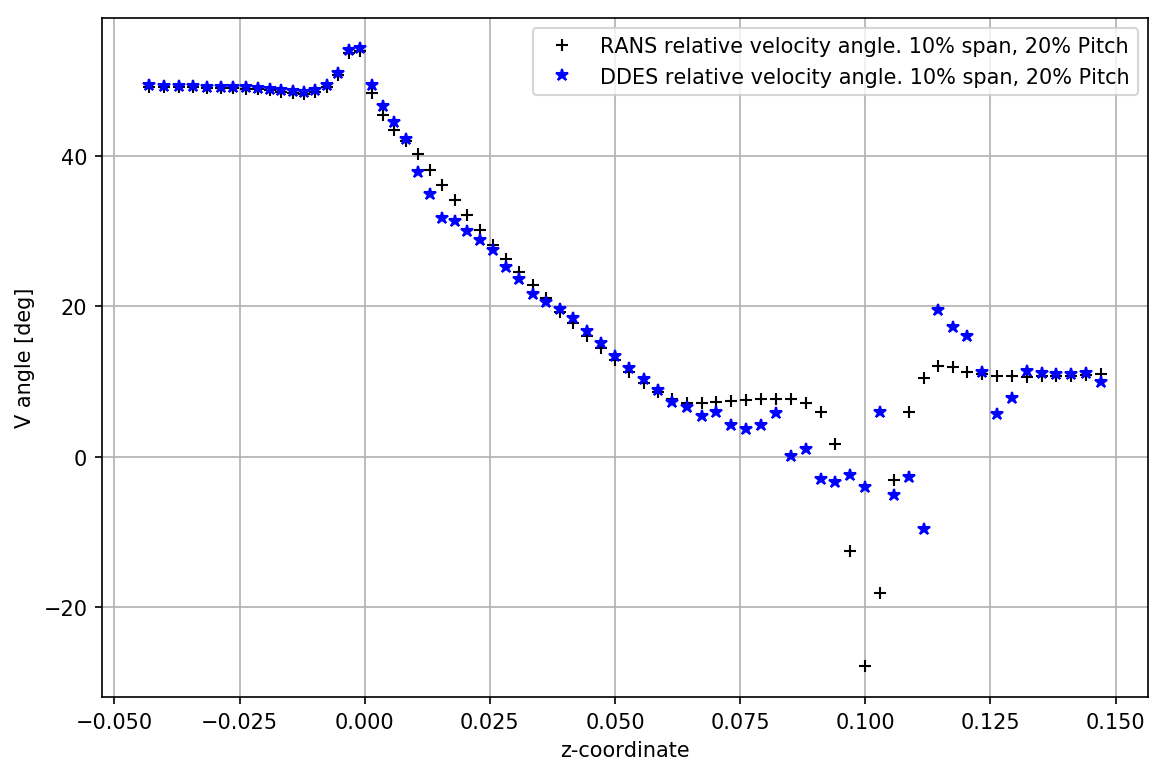
\includegraphics[width=0.7\textwidth]{Pictures/vang-rel-S10-P20.png}
  \caption{Relative velocity angle at S10P20 streamline} \label{vang-rel-S10-P20}
\end{figure}

%S10P50
\begin{figure}[ht]
  \centering
  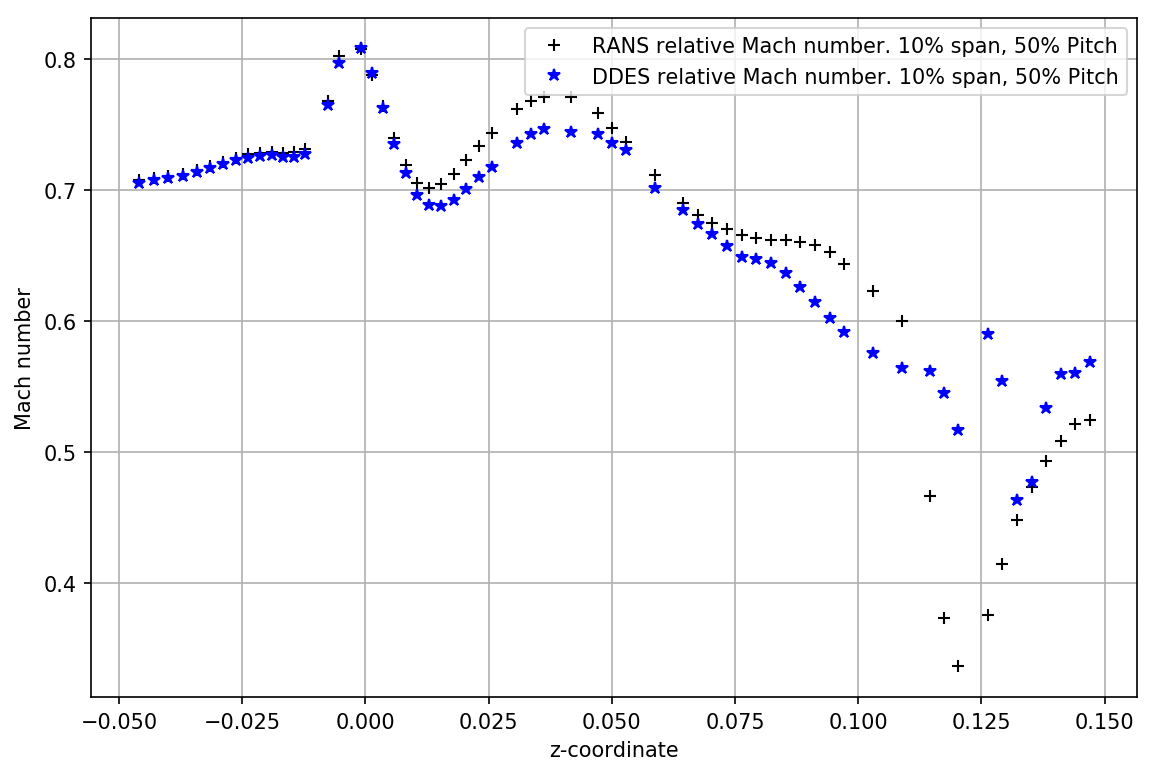
\includegraphics[width=0.75\textwidth]{Pictures/mach-rel-S10-P50.png}
  \caption{Relative Mach number at S10P50 streamline} \label{mach-rel-S10-P50}
  \vspace*{\floatsep}% https://tex.stackexchange.com/q/26521/5764
  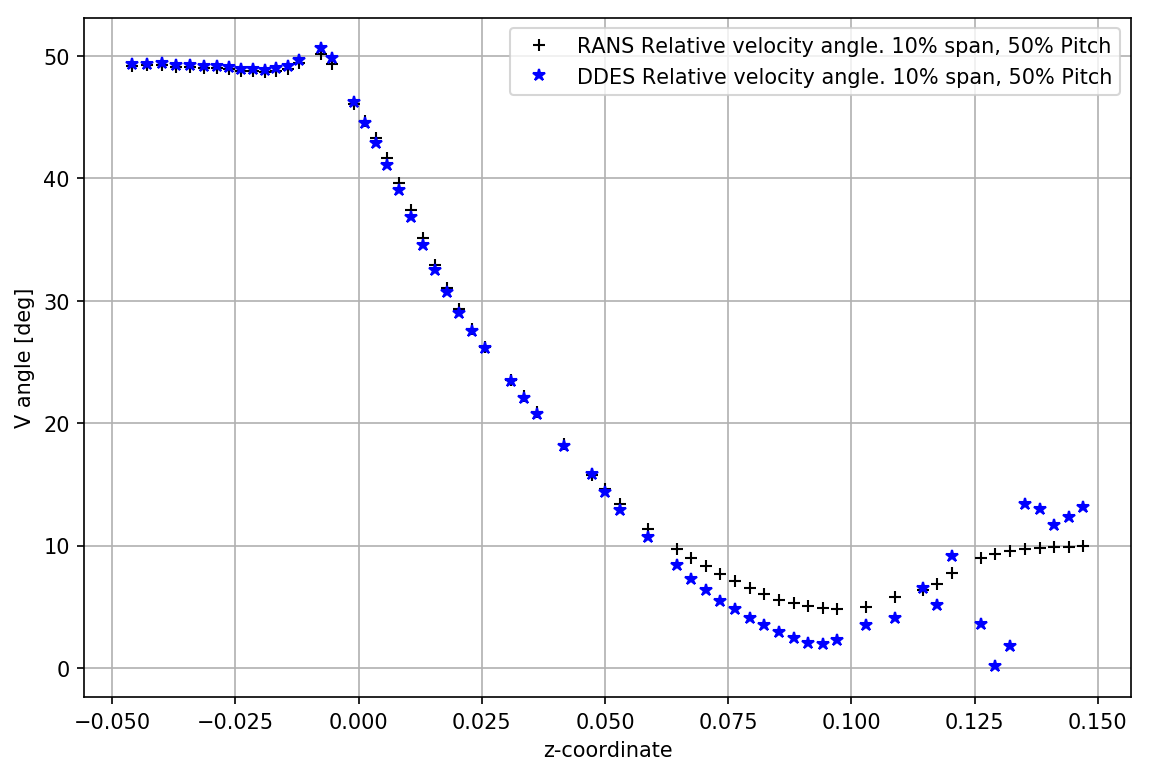
\includegraphics[width=0.75\textwidth]{Pictures/vang-rel-S10-P50.png}
  \caption{Relative velocity angle at S10P50 streamline} \label{vang-rel-S10-P50}
\end{figure}

%S10P80
\begin{figure}[ht]
  \centering
  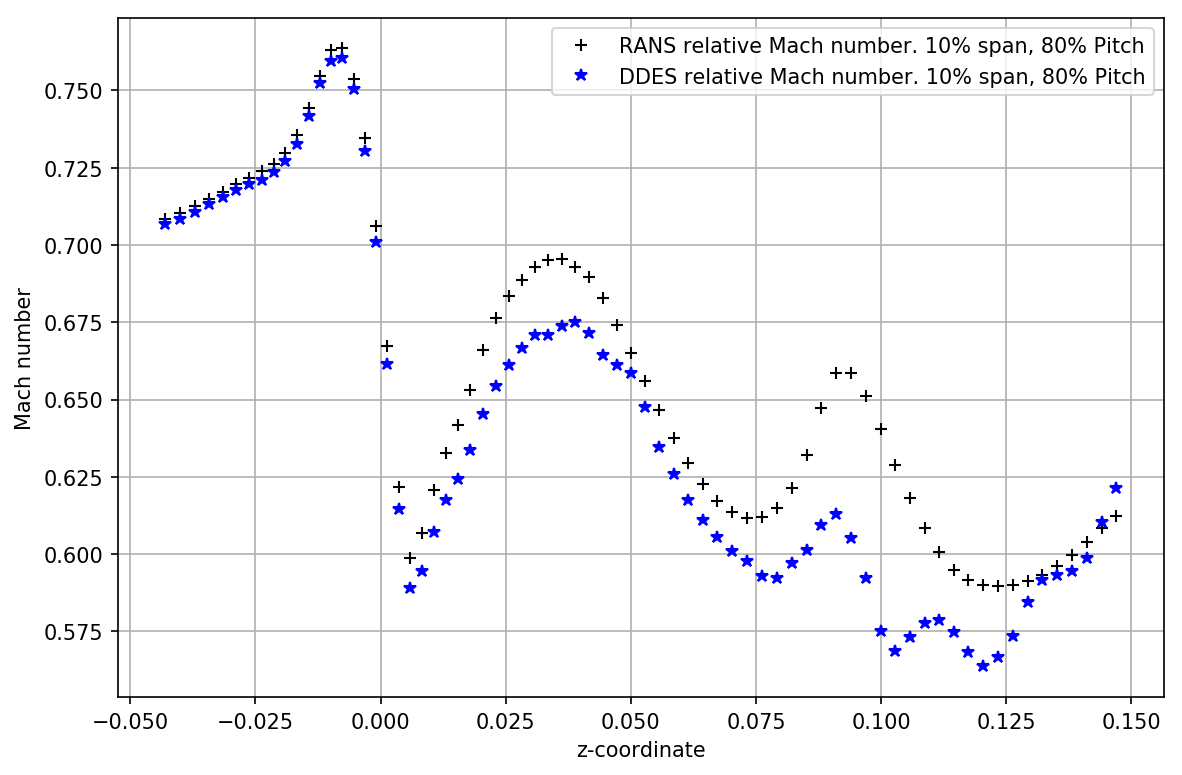
\includegraphics[width=0.75\textwidth]{Pictures/mach-rel-S10-P80.png}
  \caption{Relative Mach number at S10P80 streamline} \label{mach-rel-S10-P80}
  \vspace*{\floatsep}% https://tex.stackexchange.com/q/26521/5764
  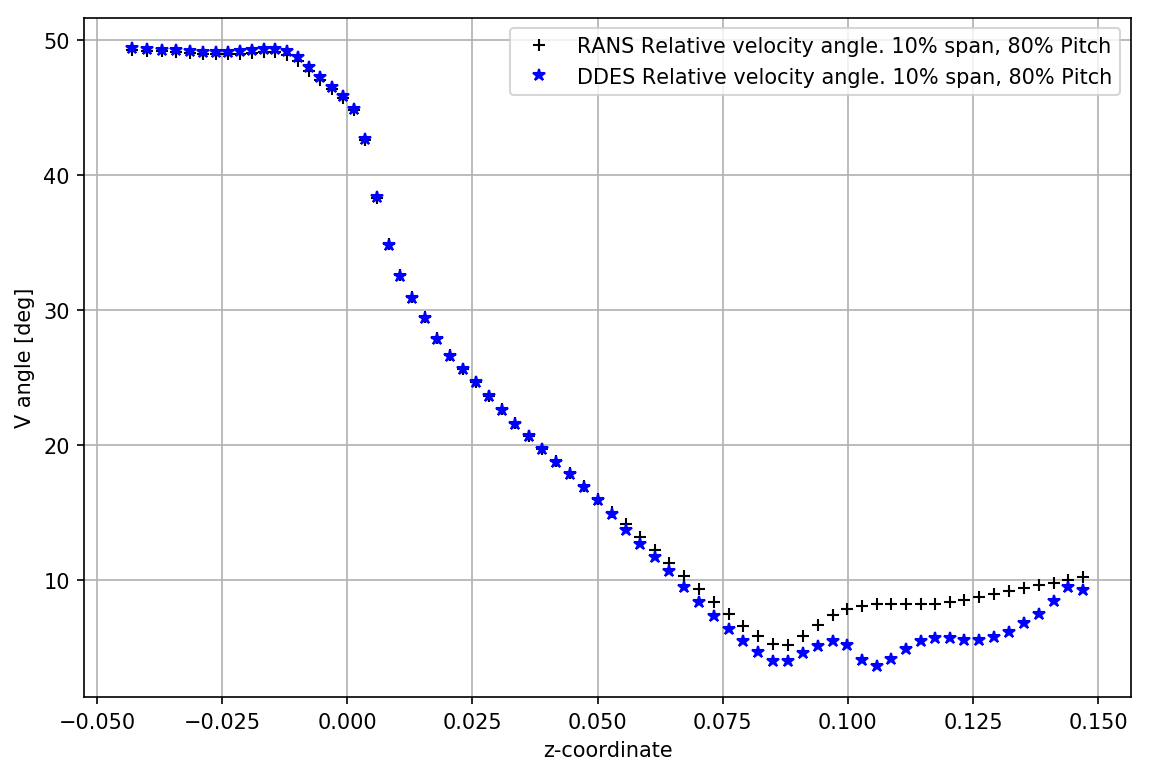
\includegraphics[width=0.75\textwidth]{Pictures/vang-rel-S10-P80.png}
  \caption{Relative velocity angle at S10P80 streamline} \label{vang-rel-S10-P80}
\end{figure}

%S50P20
\begin{figure}[ht]
  \centering
  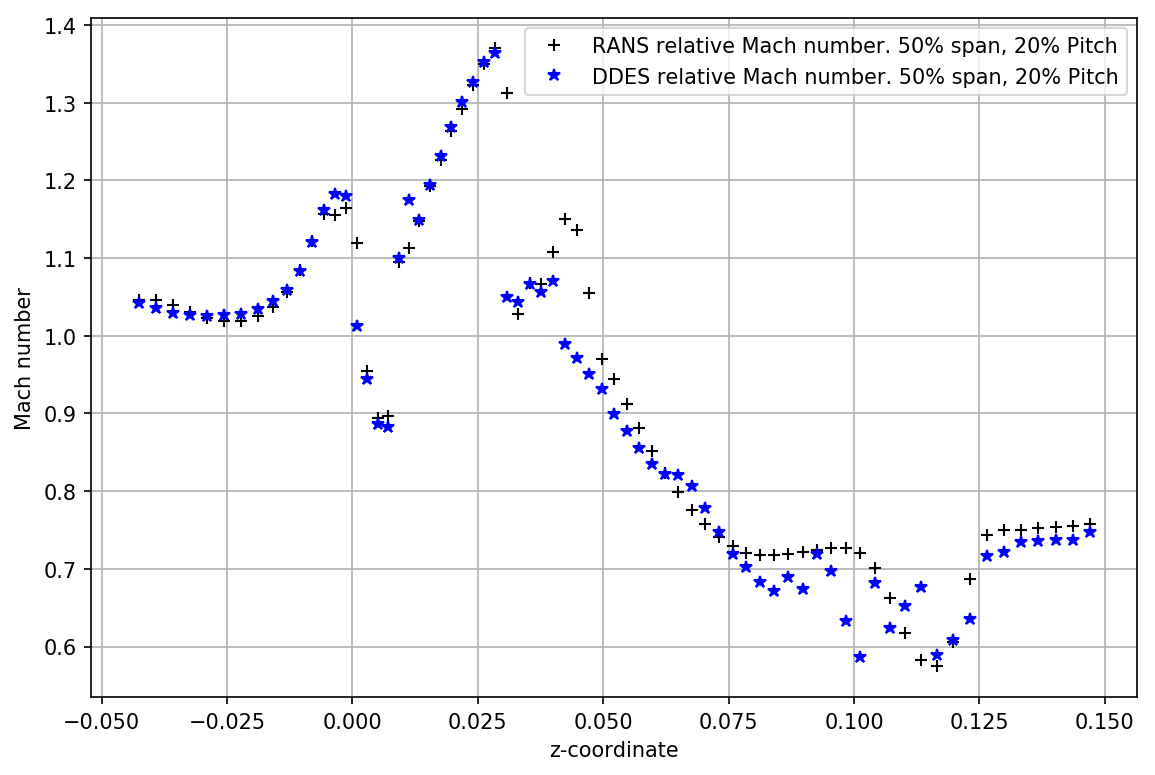
\includegraphics[width=0.75\textwidth]{Pictures/mach-rel-S50-P20.png}
  \caption{Relative Mach number at S50P20 streamline} \label{mach-rel-S50-P20}
  \vspace*{\floatsep}% https://tex.stackexchange.com/q/26521/5764
  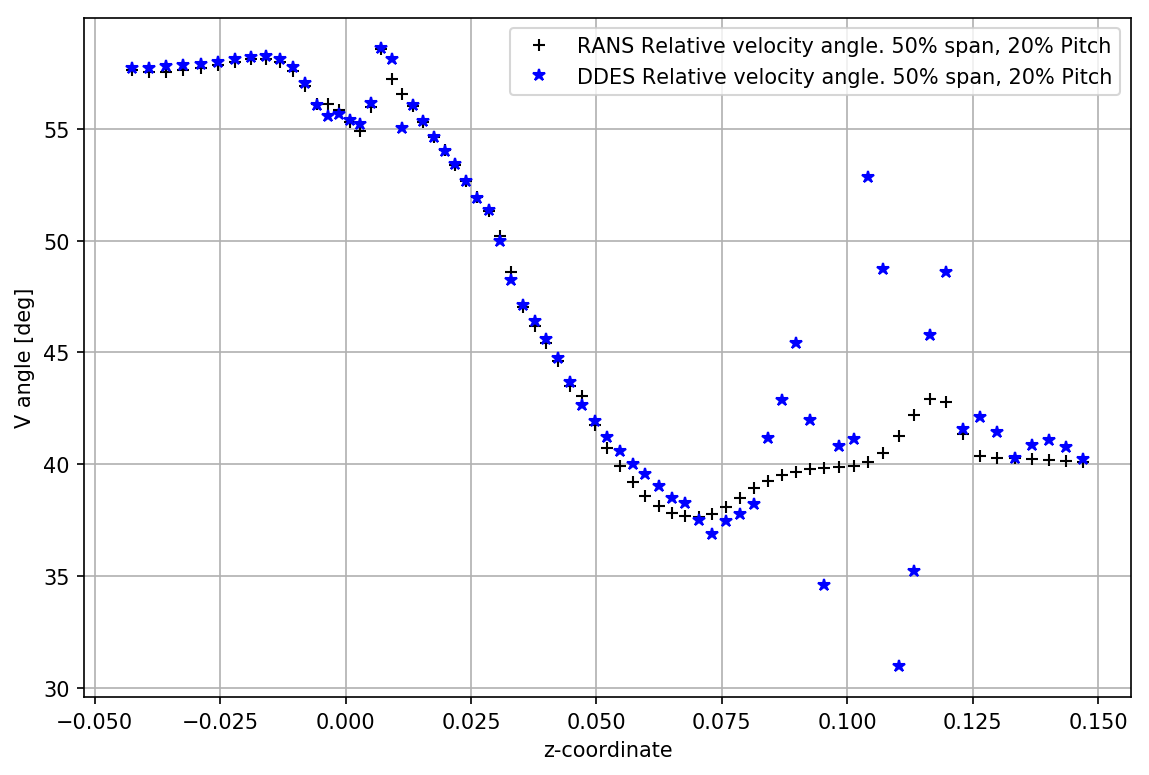
\includegraphics[width=0.75\textwidth]{Pictures/vang-rel-S50-P20.png}
  \caption{Relative velocity angle at S50P20 streamline} \label{vang-rel-S50-P20}
\end{figure}

%S50P50
\begin{figure}[ht]
  \centering
  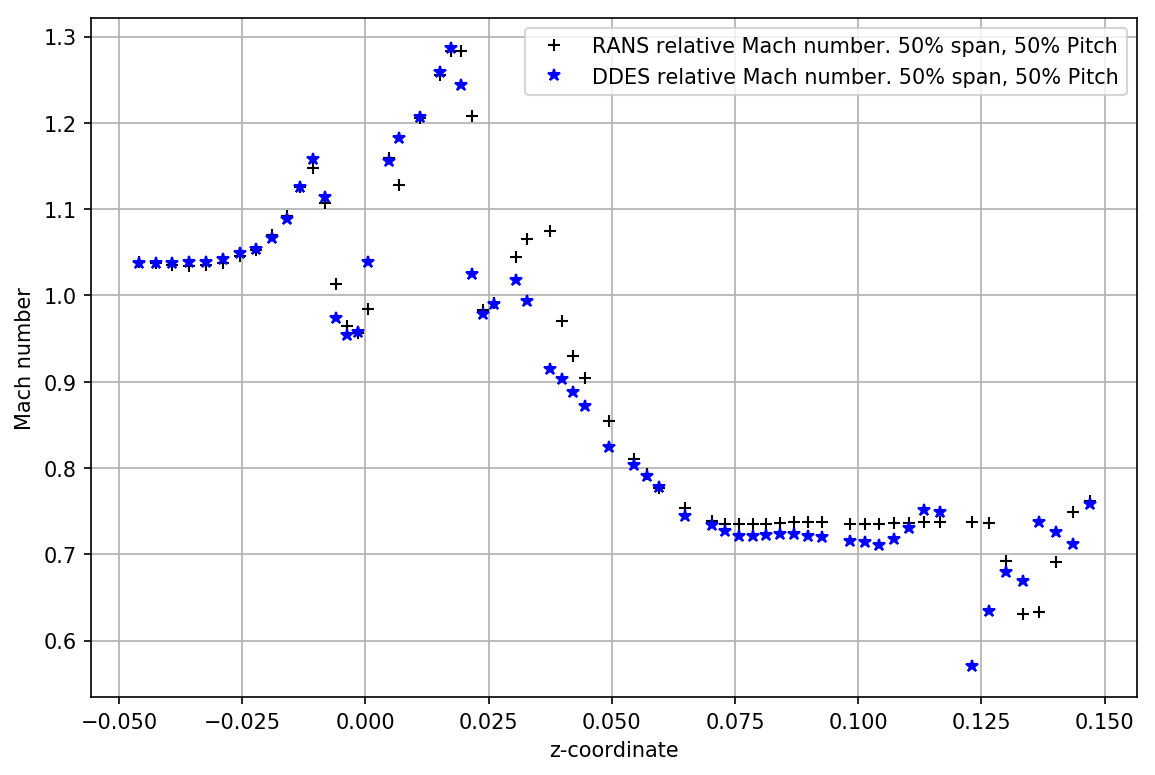
\includegraphics[width=0.75\textwidth]{Pictures/mach-rel-S50-P50.png}
  \caption{Relative Mach number at S50P50 streamline} \label{mach-rel-S50-P50}
  \vspace*{\floatsep}% https://tex.stackexchange.com/q/26521/5764
  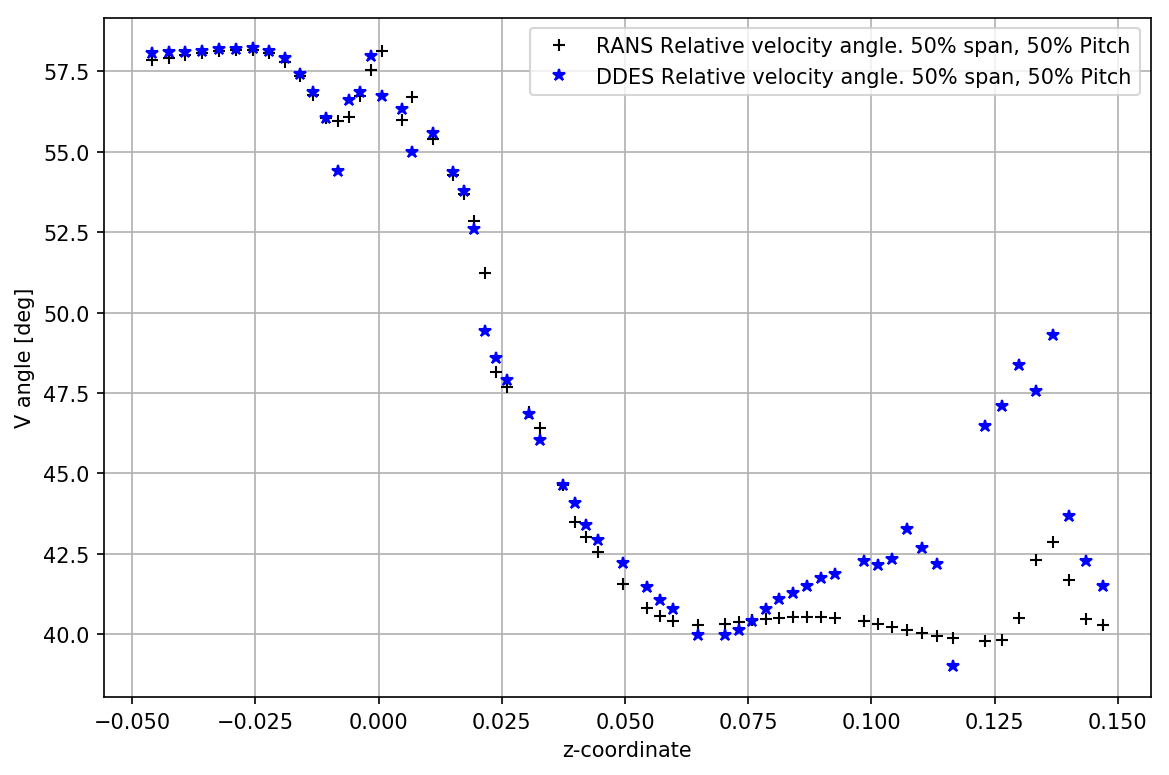
\includegraphics[width=0.75\textwidth]{Pictures/vang-rel-S50-P50.png}
  \caption{Relative velocity angle at S50P50 streamline} \label{vang-rel-S50-P50}
\end{figure}

%S50P80
\begin{figure}[ht]
  \centering
  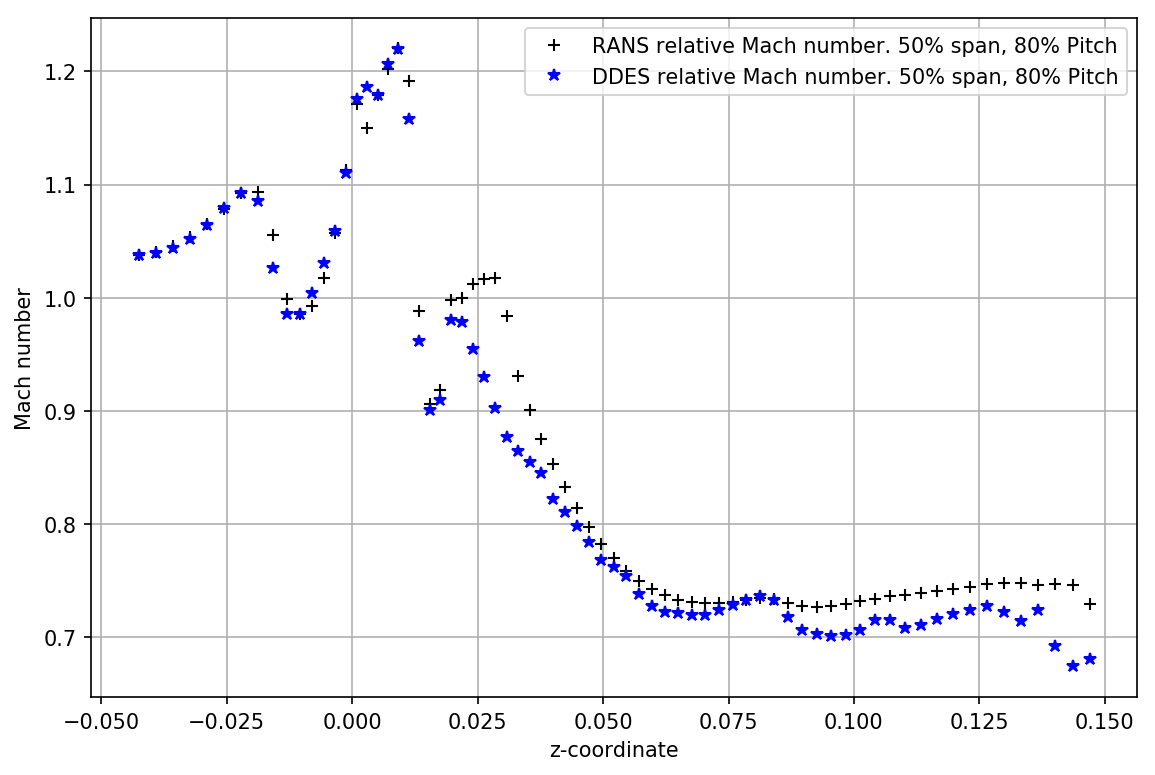
\includegraphics[width=0.75\textwidth]{Pictures/mach-rel-S50-P80.png}
  \caption{Relative Mach number at S50P80 streamline} \label{mach-rel-S50-P80}
  \vspace*{\floatsep}% https://tex.stackexchange.com/q/26521/5764
  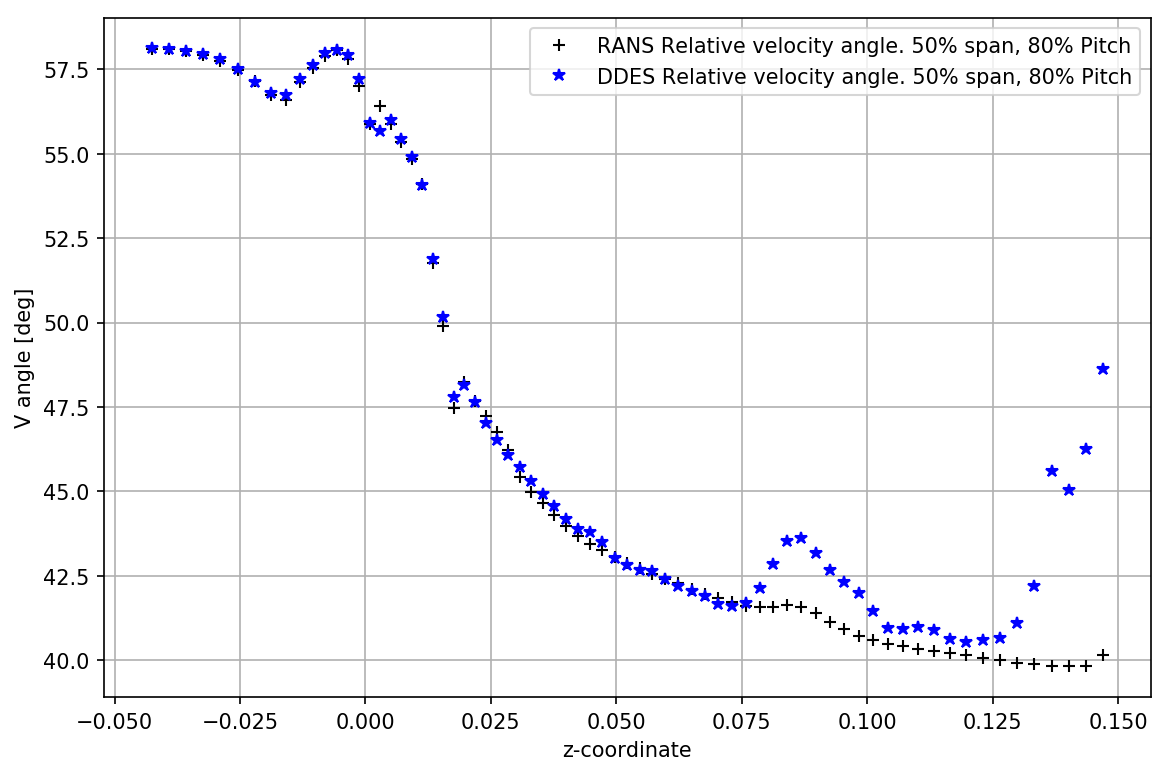
\includegraphics[width=0.75\textwidth]{Pictures/vang-rel-S50-P80.png}
  \caption{Relative velocity angle at S50P80 streamline} \label{vang-rel-S50-P80}
\end{figure}

%S90P20
\begin{figure}[ht]
  \centering
  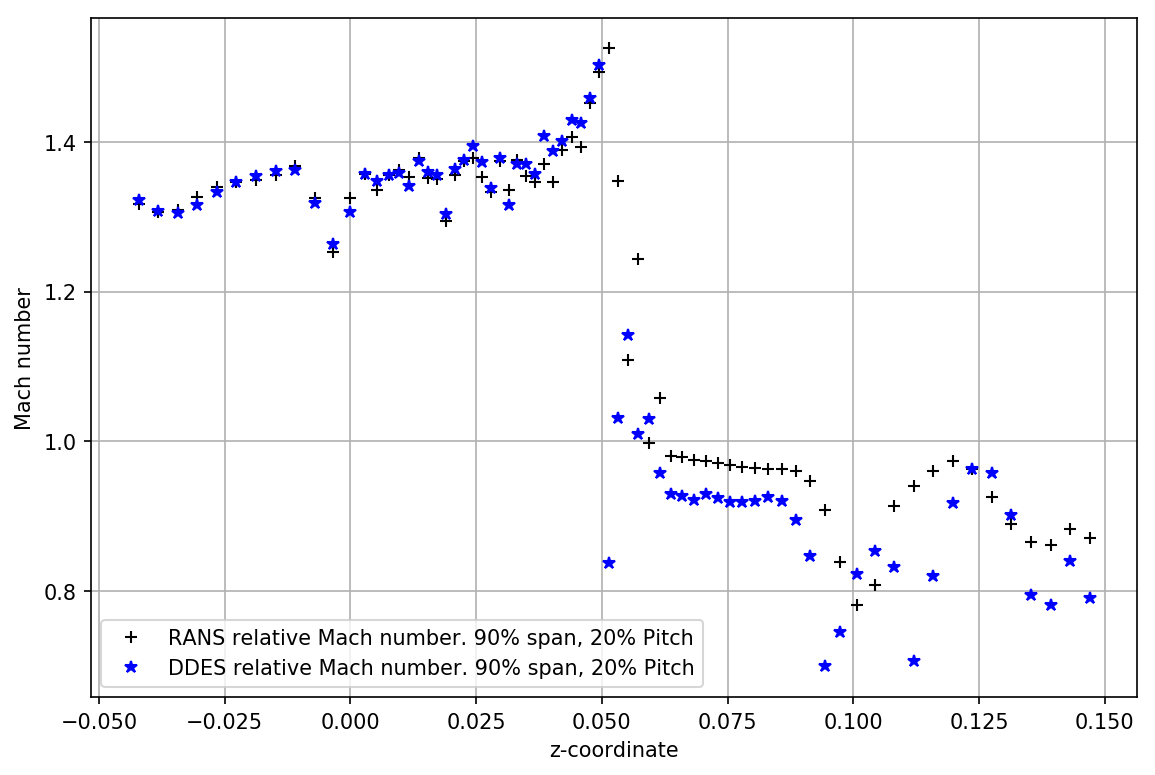
\includegraphics[width=0.75\textwidth]{Pictures/mach-rel-S90-P20.png}
  \caption{Relative Mach number at S90P20 streamline} \label{mach-rel-S90-P20}
  \vspace*{\floatsep}% https://tex.stackexchange.com/q/26521/5764
  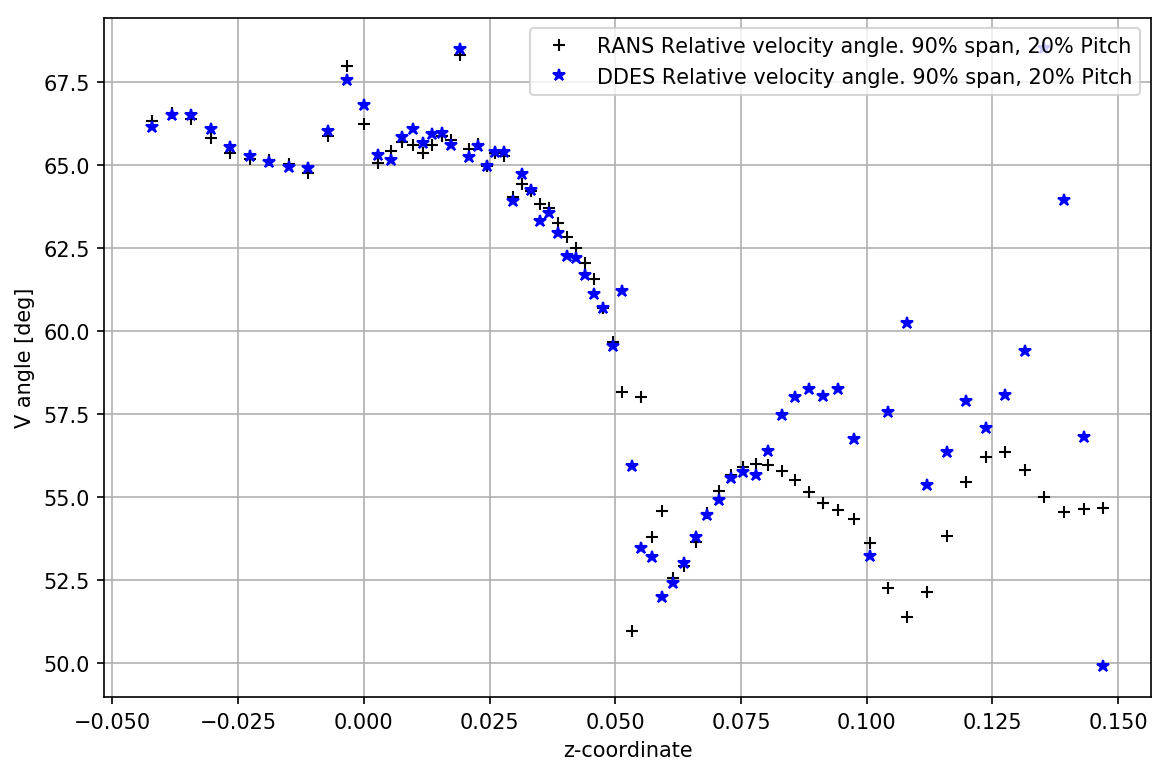
\includegraphics[width=0.75\textwidth]{Pictures/vang-rel-S90-P20.png}
  \caption{Relative velocity angle at S90P20 streamline} \label{vang-rel-S90-P20}
\end{figure}

%S90P50
\begin{figure}[ht]
  \centering
  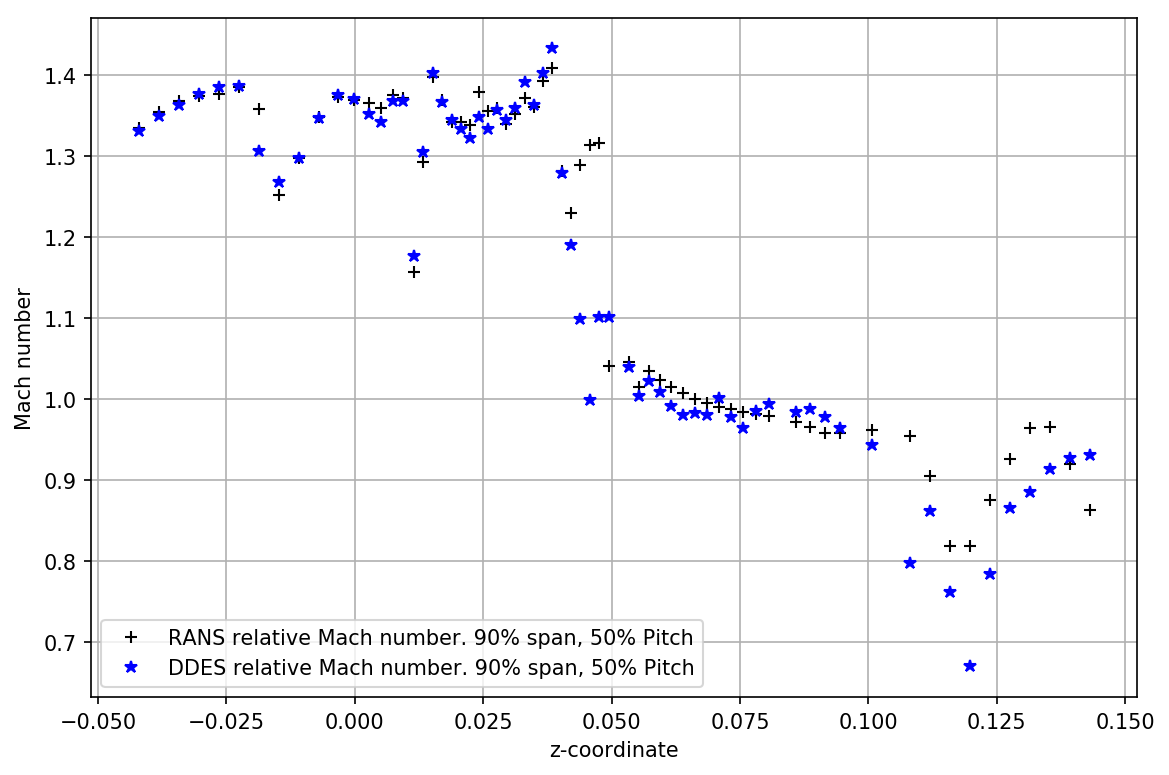
\includegraphics[width=0.75\textwidth]{Pictures/mach-rel-S90-P50.png}
  \caption{Relative Mach number at S90P50 streamline} \label{mach-rel-S90-P50}
  \vspace*{\floatsep}% https://tex.stackexchange.com/q/26521/5764
  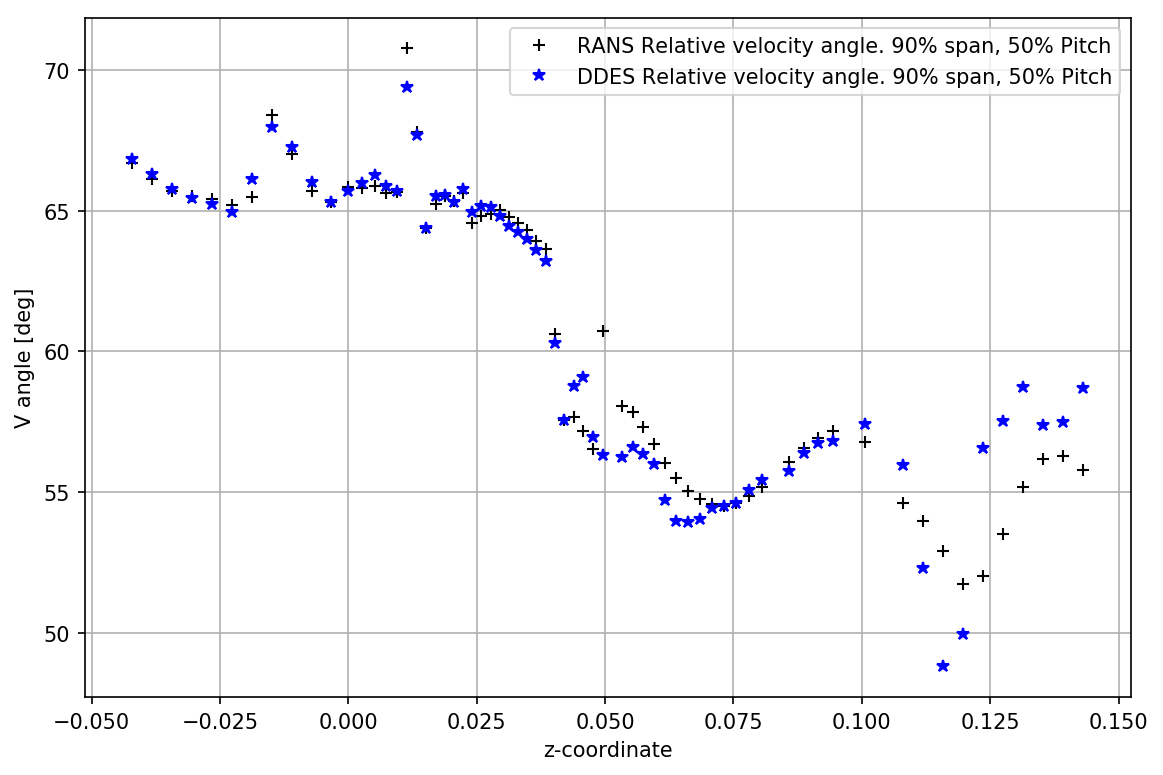
\includegraphics[width=0.75\textwidth]{Pictures/vang-rel-S90-P50.png}
  \caption{Relative velocity angle at S90P50 streamline} \label{vang-rel-S90-P50}
\end{figure}

%S90P80
\begin{figure}[ht]
  \centering
  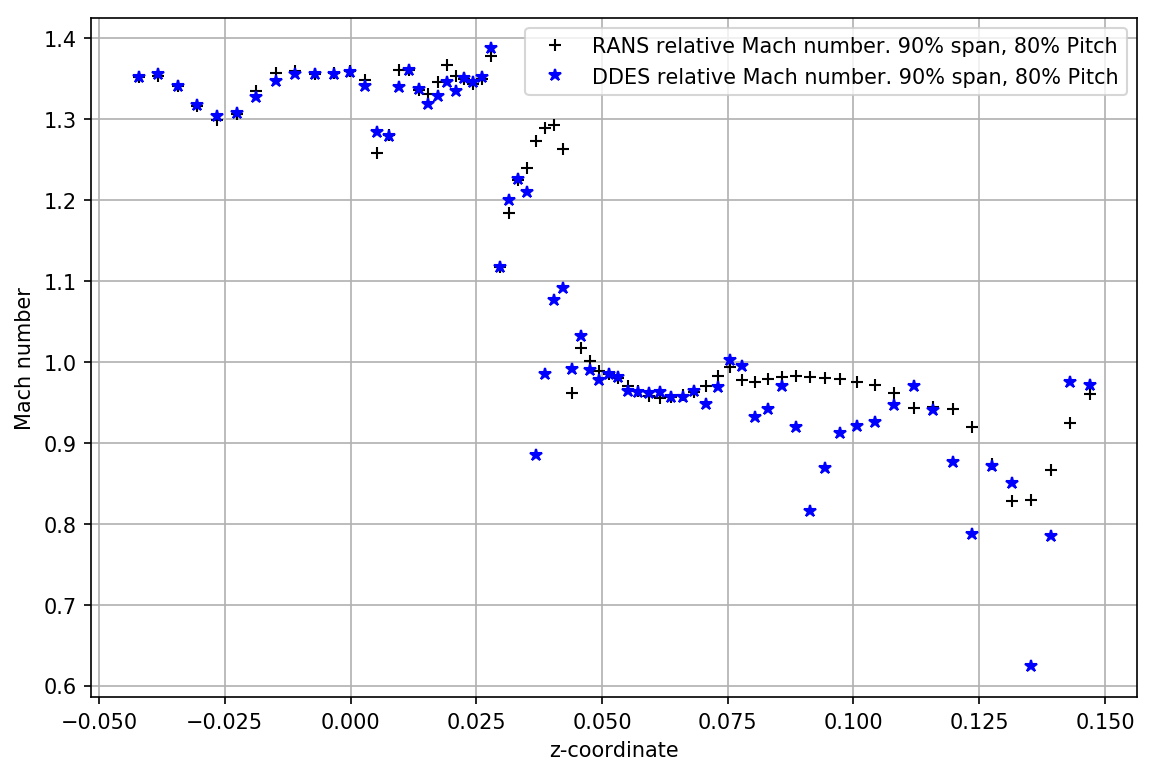
\includegraphics[width=0.75\textwidth]{Pictures/mach-rel-S90-P80.png}
  \caption{Relative Mach number at S90P80 streamline} \label{mach-rel-S90-P80}
  \vspace*{\floatsep}% https://tex.stackexchange.com/q/26521/5764
  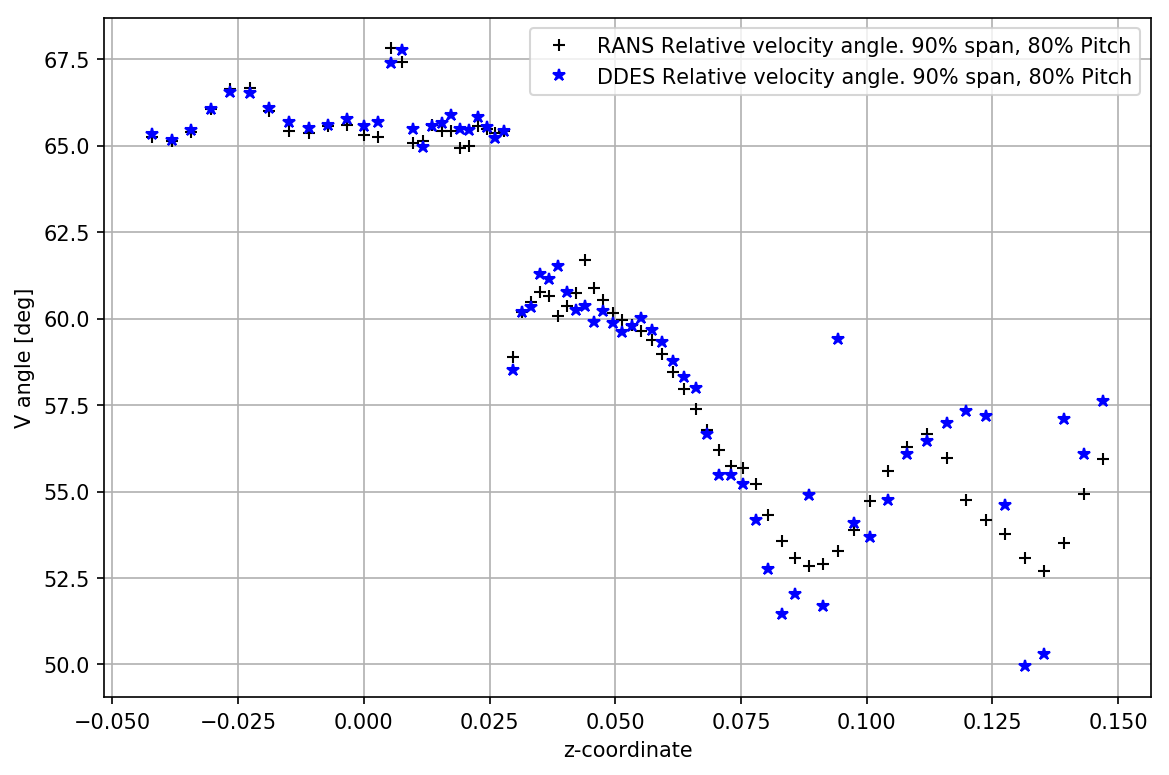
\includegraphics[width=0.75\textwidth]{Pictures/vang-rel-S90-P80.png}
  \caption{Relative velocity angle at S90P80 streamline} \label{vang-rel-S90-P80}
\end{figure}

%int-01
\begin{figure}[ht]
  \centering
%  
\includegraphics[width=0.5\textwidth]{Pictures/placeholder.jpg}
%  \caption{Mach number contour plot @10\% span \citep{r67laser}} \label{10-mach-exp}
%  
%  \vspace*{\floatsep}% https://tex.stackexchange.com/q/26521/5764

  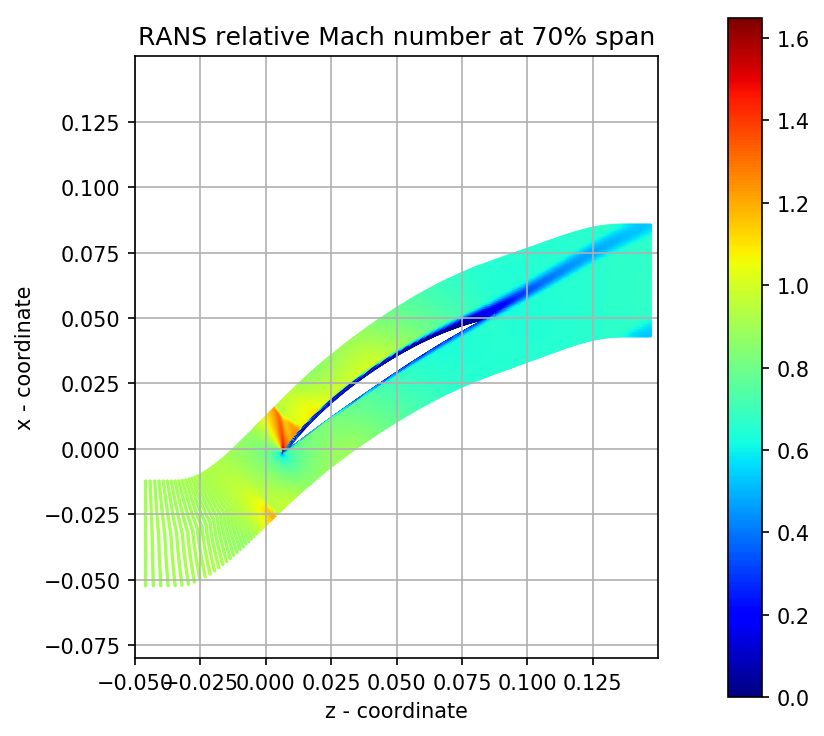
\includegraphics[width=0.75\textwidth]{Pictures/rans-mach-int-04.png}
  \caption{RANS Mach number contour plot at int-04 mark} \label{int-04-rans-mach}
  
   \vspace*{\floatsep}% https://tex.stackexchange.com/q/26521/5764
   
  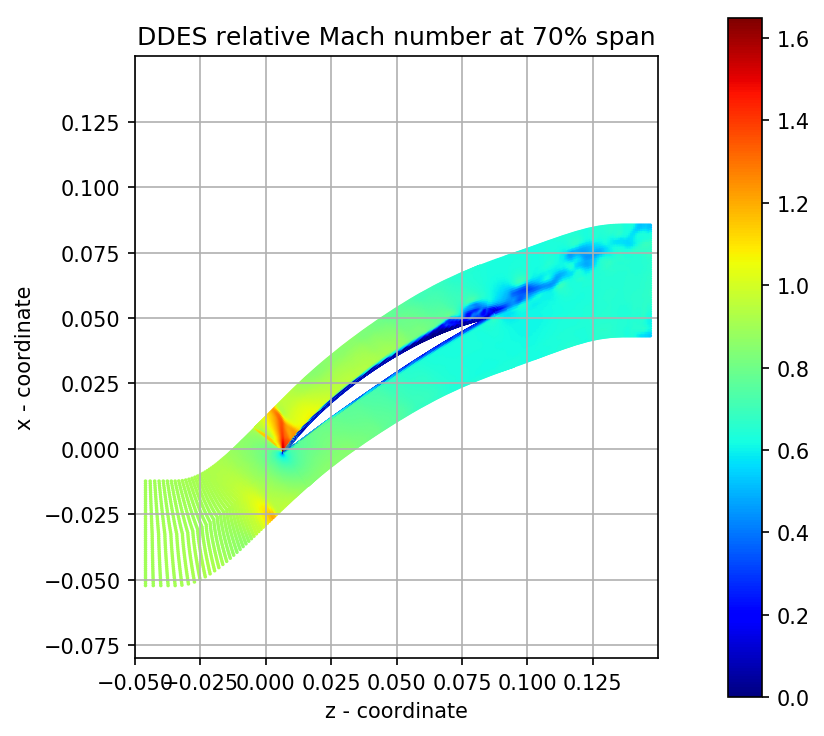
\includegraphics[width=0.75\textwidth]{Pictures/ddes-mach-int-04.png}
  \caption{DDES Mach number contour plot at int-04 mark} \label{int-04-ddes-mach}
\end{figure}

%int-07
\begin{figure}[ht]
  \centering
%  
\includegraphics[width=0.5\textwidth]{Pictures/placeholder.jpg}
%  \caption{Mach number contour plot @10\% span \citep{r67laser}} \label{10-mach-exp}
%  
%  \vspace*{\floatsep}% https://tex.stackexchange.com/q/26521/5764

  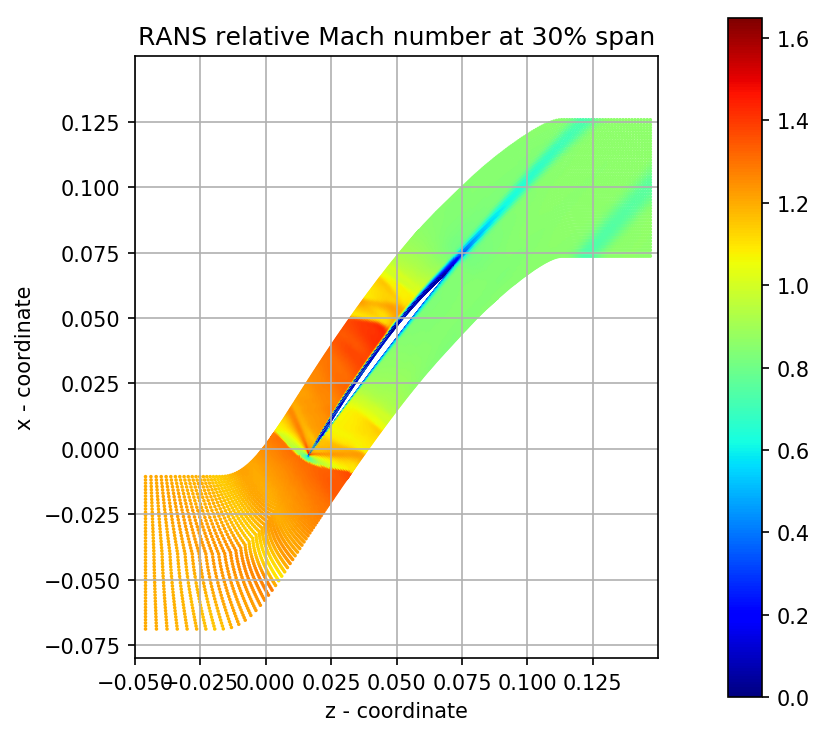
\includegraphics[width=0.75\textwidth]{Pictures/rans-mach-int-09.png}
  \caption{RANS Mach number contour plot at int-09 mark} \label{int-09-rans-mach}
  
   \vspace*{\floatsep}% https://tex.stackexchange.com/q/26521/5764
   
  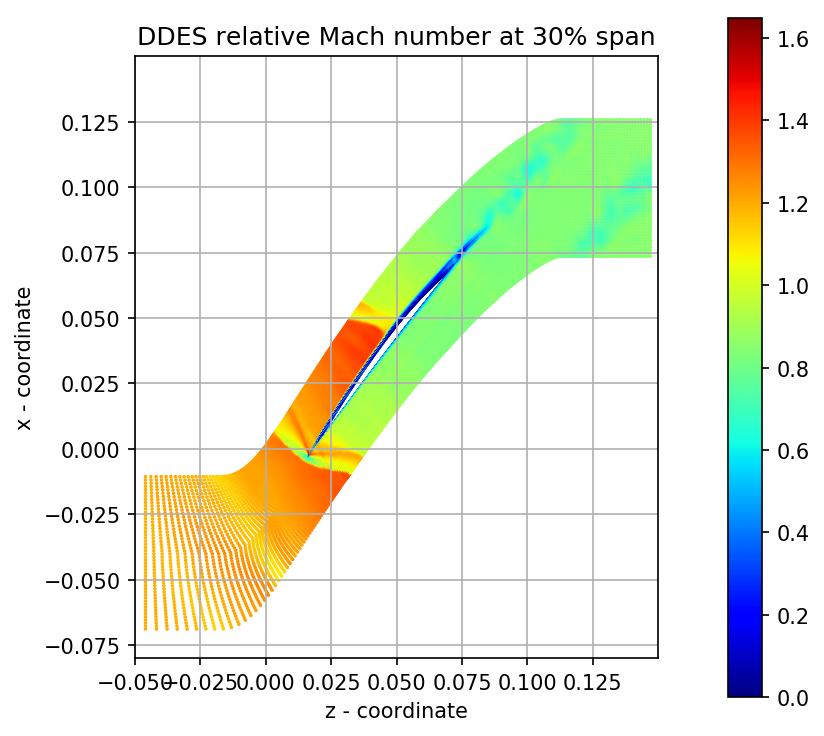
\includegraphics[width=0.75\textwidth]{Pictures/ddes-mach-int-09.png}
  \caption{DDES Mach number contour plot at int-09 mark} \label{int-09-ddes-mach}
\end{figure}

%int-12
\begin{figure}[ht]
  \centering
%  
\includegraphics[width=0.5\textwidth]{Pictures/placeholder.jpg}
%  \caption{Mach number contour plot @10\% span \citep{r67laser}} \label{10-mach-exp}
%  
%  \vspace*{\floatsep}% https://tex.stackexchange.com/q/26521/5764

  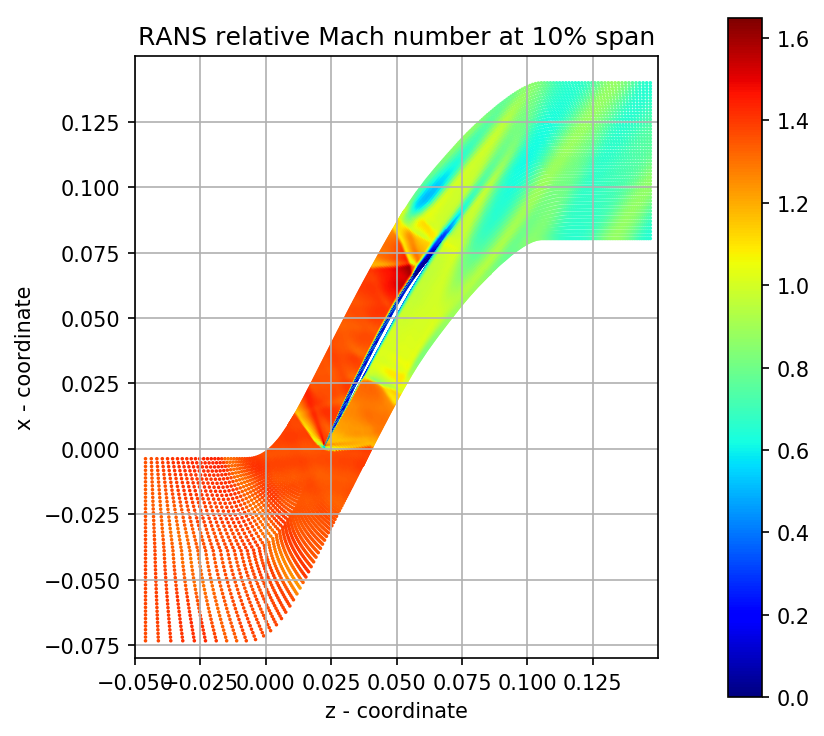
\includegraphics[width=0.75\textwidth]{Pictures/rans-mach-int-12.png}
  \caption{RANS Mach number contour plot at int-12 mark} \label{int-12-rans-mach}
  
   \vspace*{\floatsep}% https://tex.stackexchange.com/q/26521/5764
   
  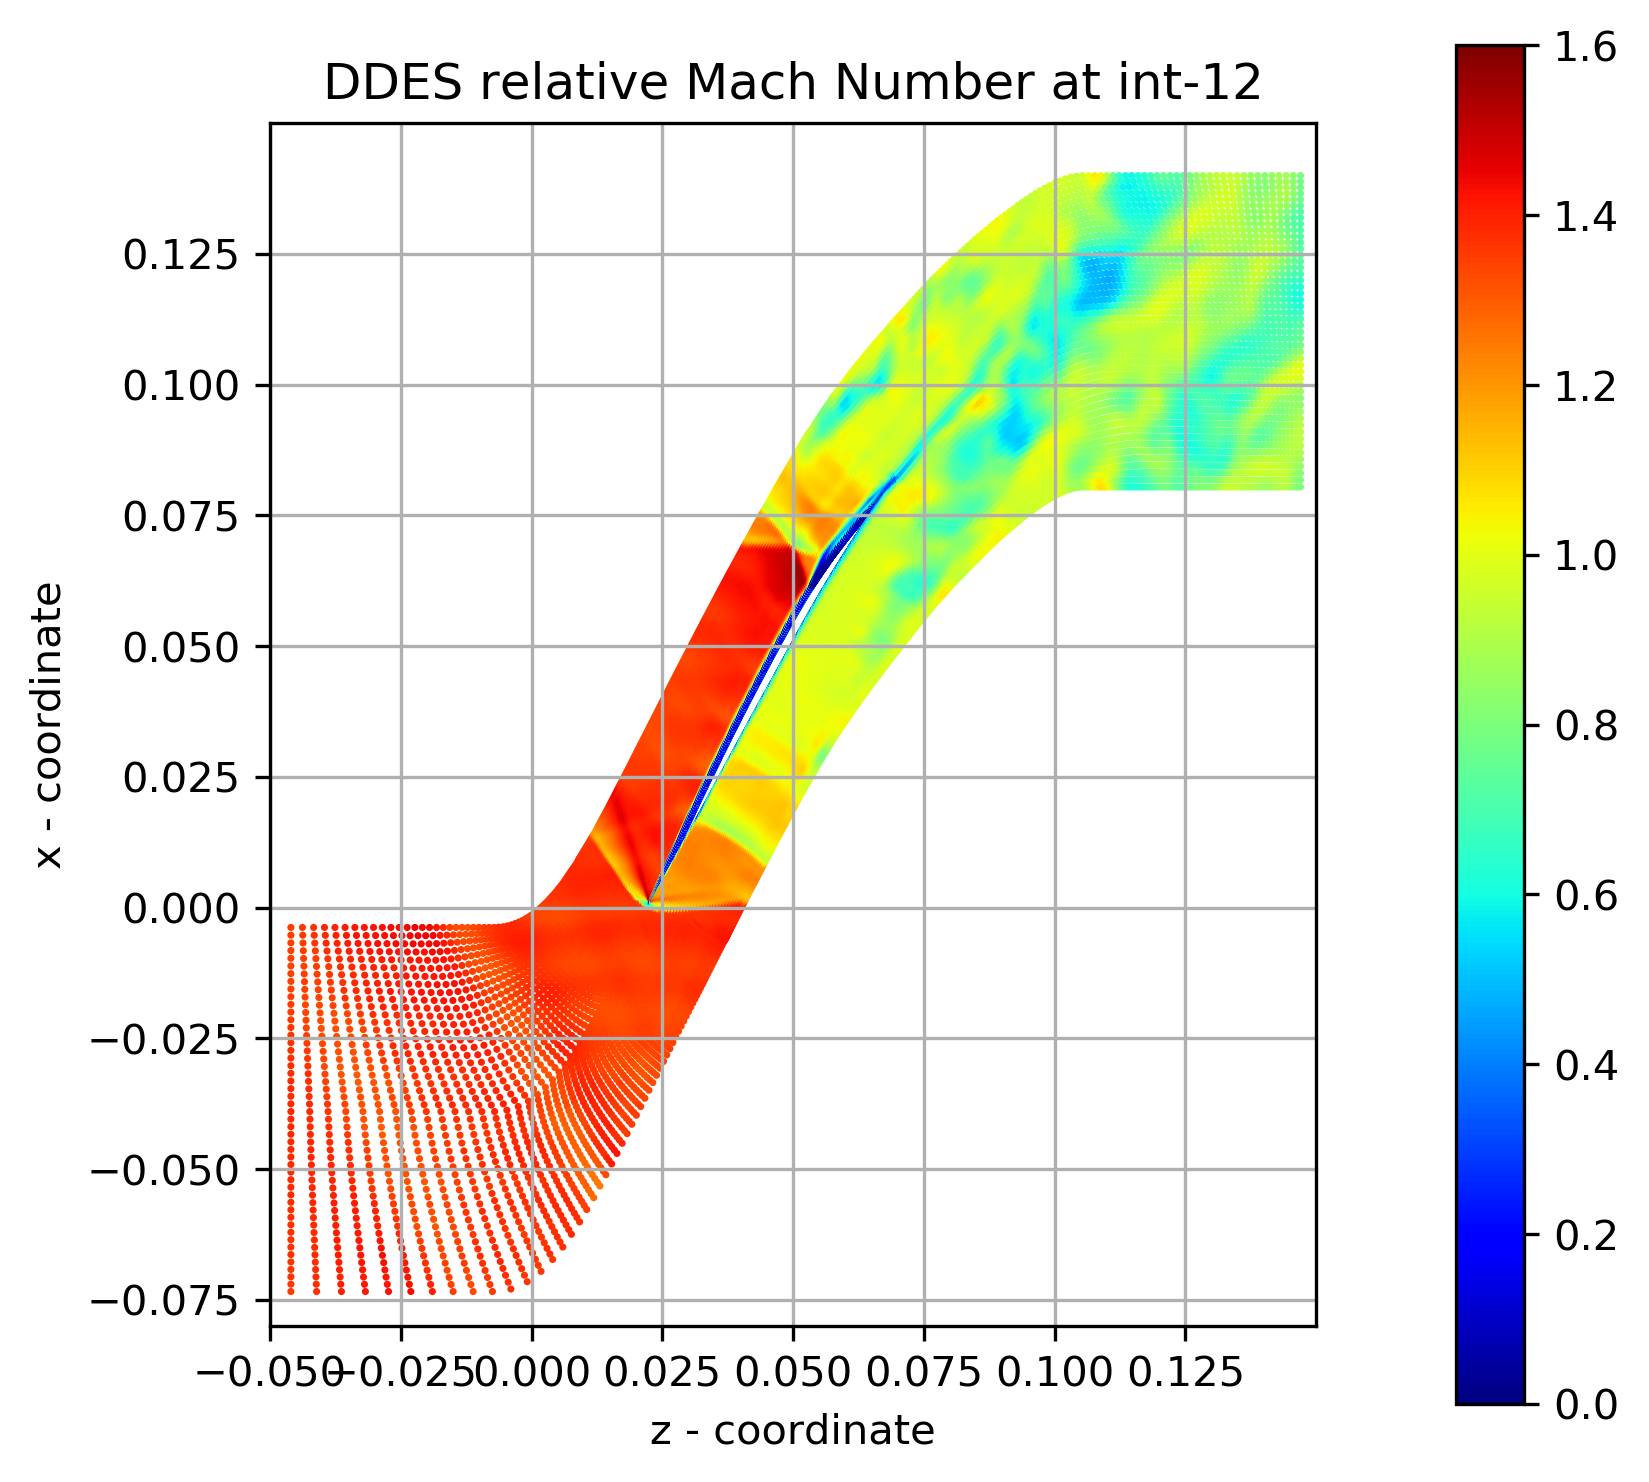
\includegraphics[width=0.75\textwidth]{Pictures/ddes-mach-int-12.png}
  \caption{DDES Mach number contour plot at int-12 mark} \label{int-12-ddes-mach}
\end{figure}